\begin{figure}
    \centering
    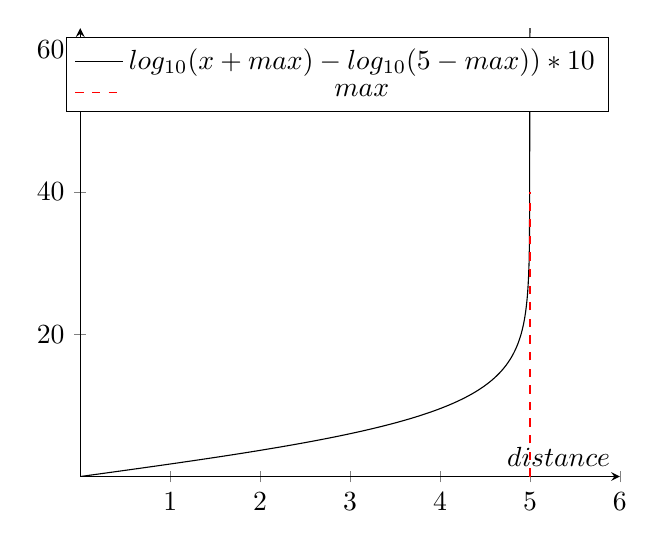
\begin{tikzpicture}
     \begin{axis}[ 
        xlabel={$distance$},
        ylabel={$force$},
        axis lines=middle,
        xmin=0,
        xmax=6,
      ] 
        \addplot[samples=1000, domain=0:5] {(log10(x + 5) - log10(5 - x))*10}; 
        \addlegendentry{$log_{10}(x + max) - log_{10}(5 - max)) * 10$}
        
        \addplot +[mark=none, dashed] coordinates {(5, 0) (5, 40)};
        \addlegendentry{$max$}
      \end{axis}
    \end{tikzpicture}

    \caption{Shows the gravity equation based on logit.}
    \label{fig:gravityPlot}
\end{figure}